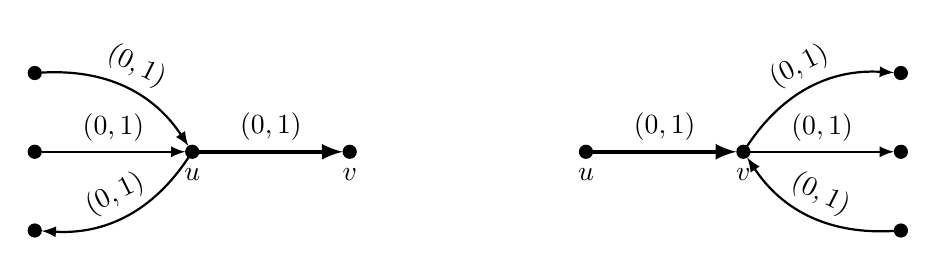
\begin{tikzpicture}[auto]

	\node (u) [circle, scale=0.5, fill, draw, label=below:$u$] at (0, 0) {};
	\node (v) [circle, scale=0.5, fill, draw, label=below:$v$] at (2, 0) {};
	\node (w1) [circle, scale=0.5, fill, draw] at (-2, -1) {};
	\node (w2) [circle, scale=0.5, fill, draw] at (-2, 0) {};
	\node (w3) [circle, scale=0.5, fill, draw] at (-2, 1) {};

	\path[thick, -latex]
	(u) edge[ultra thick] node[sloped] {$(0,1)$} (v)
	(u) edge[bend left] node[sloped] {$(0,1)$} (w1)
	(w3) edge[bend left] node[sloped] {$(0,1)$} (u)
	(w2) edge node[sloped] {$(0,1)$} (u);

	\node (v') [circle, scale=0.5, fill, draw, label=below:$v$] at (7, 0) {};
	\node (u') [circle, scale=0.5, fill, draw, label=below:$u$] at (5, 0) {};
	\node (w1') [circle, scale=0.5, fill, draw] at (9, -1) {};
	\node (w2') [circle, scale=0.5, fill, draw] at (9, 0) {};
	\node (w3') [circle, scale=0.5, fill, draw] at (9, 1) {};

	\path[thick, -latex]
	(u') edge[ultra thick] node[sloped] {$(0,1)$} (v')
	(w1') edge[bend left] node[sloped] {$(0,1)$} (v')
	(v') edge[bend left] node[sloped] {$(0,1)$} (w3')
	(v') edge node[sloped] {$(0,1)$} (w2');

\end{tikzpicture}
